\chapter{Refactoring}

\section{Code Smells}
\begin{lstlisting}[
	captionpos=b,
	caption={Beschreibung eines in einem Bild enthaltenen Objektes mittels des Yolo Datei Formats},
	label={code:LongParameterList},
	language=java,
	escapeinside={@}{@}]
	public RPGCharacter(CharacterRace race, CharacterClass characterClass, Background background, Inventory inventory, String name, Attributes attributes, DeathSaves deathSaves, Player player, int xp, int age) throws RPGCharacterException
\end{lstlisting}
Listing \ref{code:LongParameterList} zeigt den Konstruktor der Klasse \texttt{RPGCharakter}. Dieser stellt den CodeSmell Long Parameter List dar. Um diesen zu lösen, müsste man mehrere der bereits zusammengefassten Objekte in weitere Objekte zusammenfassen. So wäre es z.B. möglich die Parameter \texttt{race}, \texttt{characterClass}, \texttt{Background}, \texttt{Attributes} in ein neues Objekt namens \texttt{CharacterProperties} zusammen zu fassen.

Die gesamte Klasse \texttt{InventoryService} besteht aus dead code. Sie wurde im Vorfeld angelegt um Änderungen im Inventory vornehmen zu können. Später wurde der Scope des Projektes jedoch verändert und der Code wird nicht mehr benötigt, wurde aber nicht gelöscht. Dementsprächend wäre es sinnvoll diesen Code nun zu löschen.

\section{2 Refactorings}
\subsection{Rename Method}
\begin{figure}[H]
	\centering
	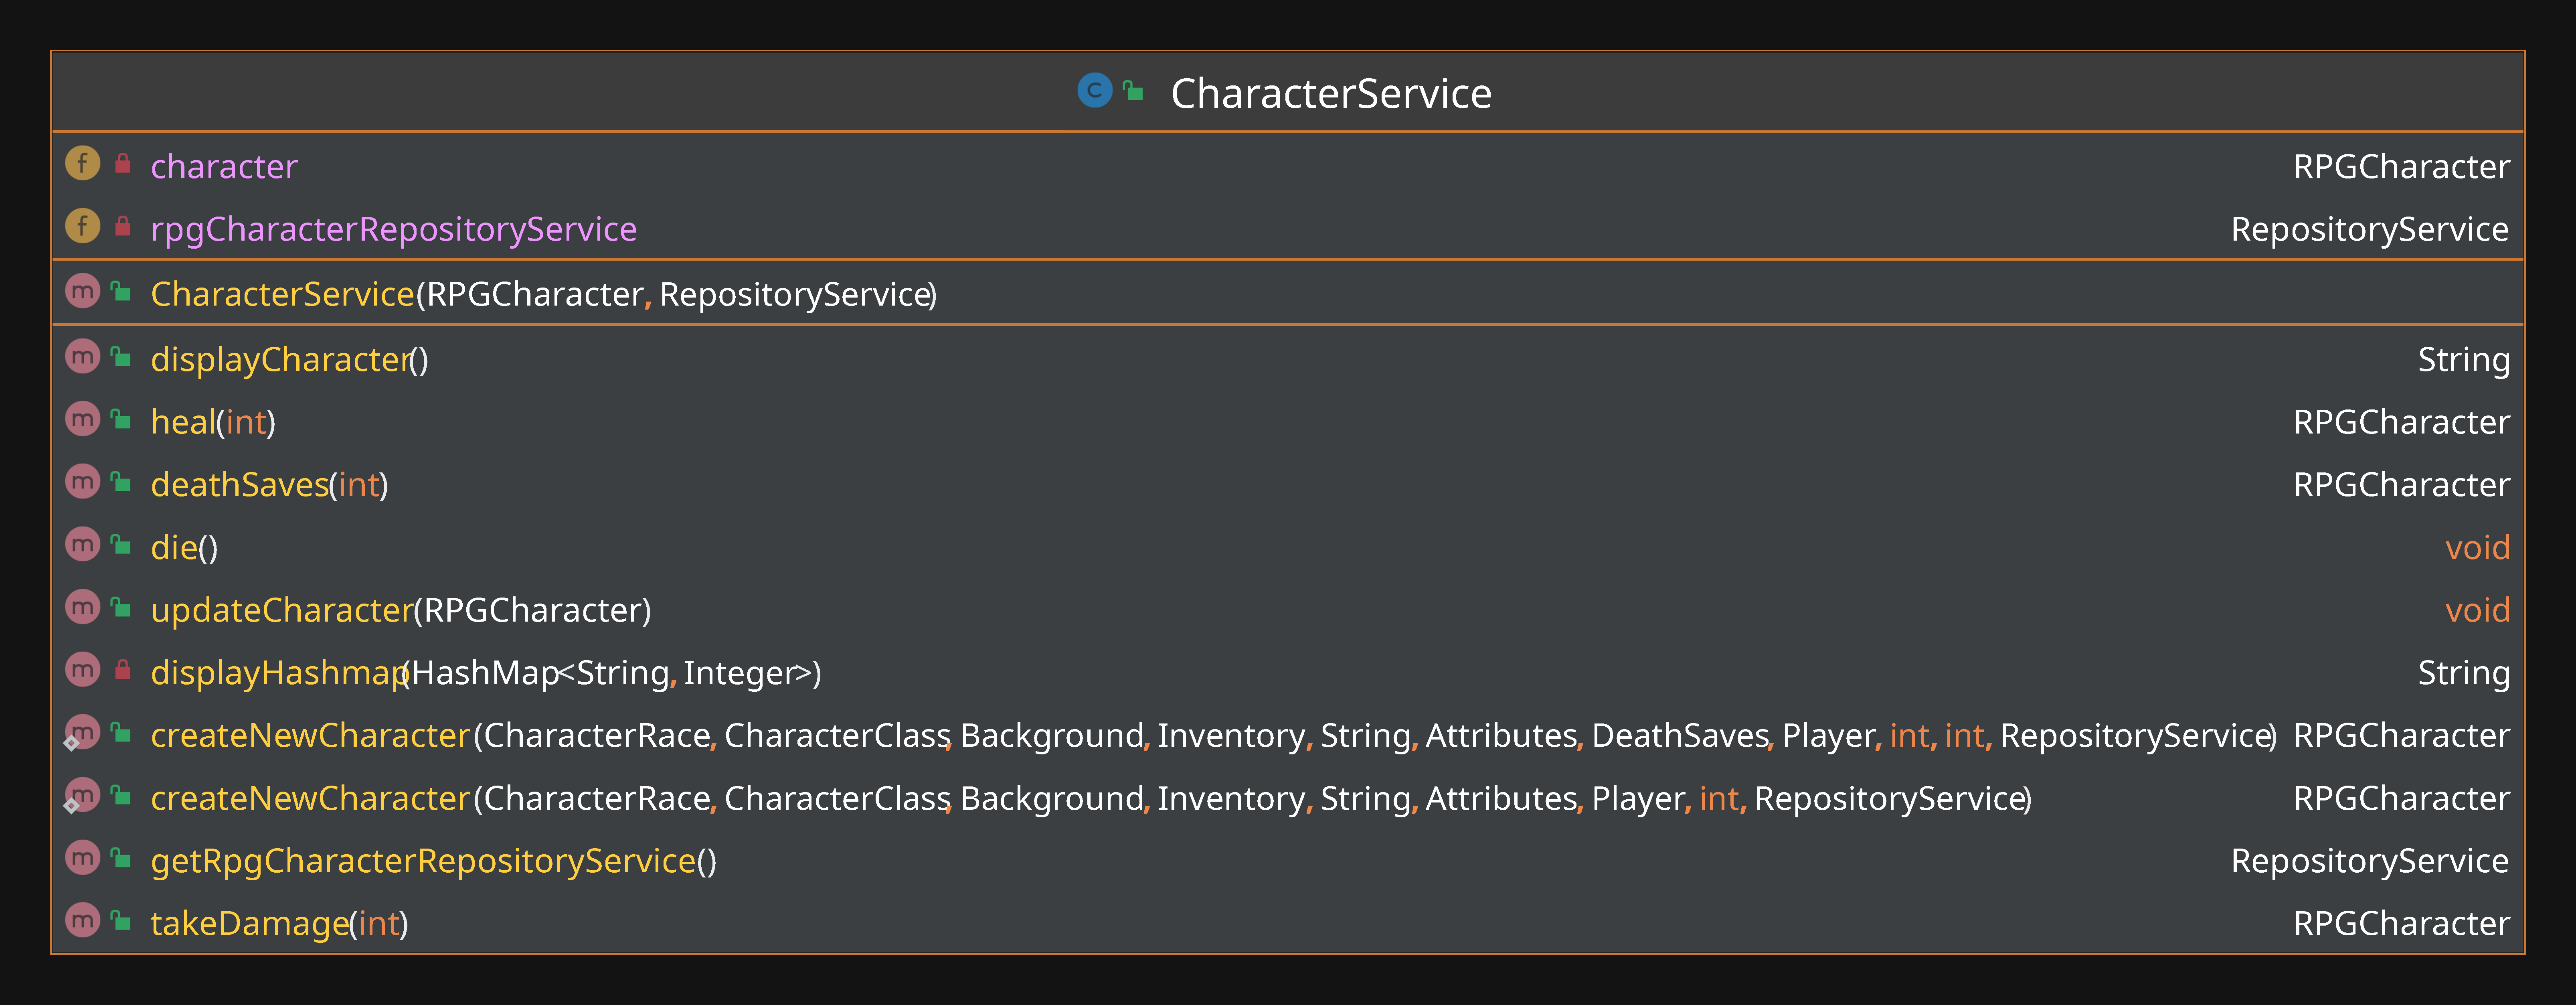
\includegraphics[width=0.49\textwidth]{Bilder/CharacterService-old.pdf}
	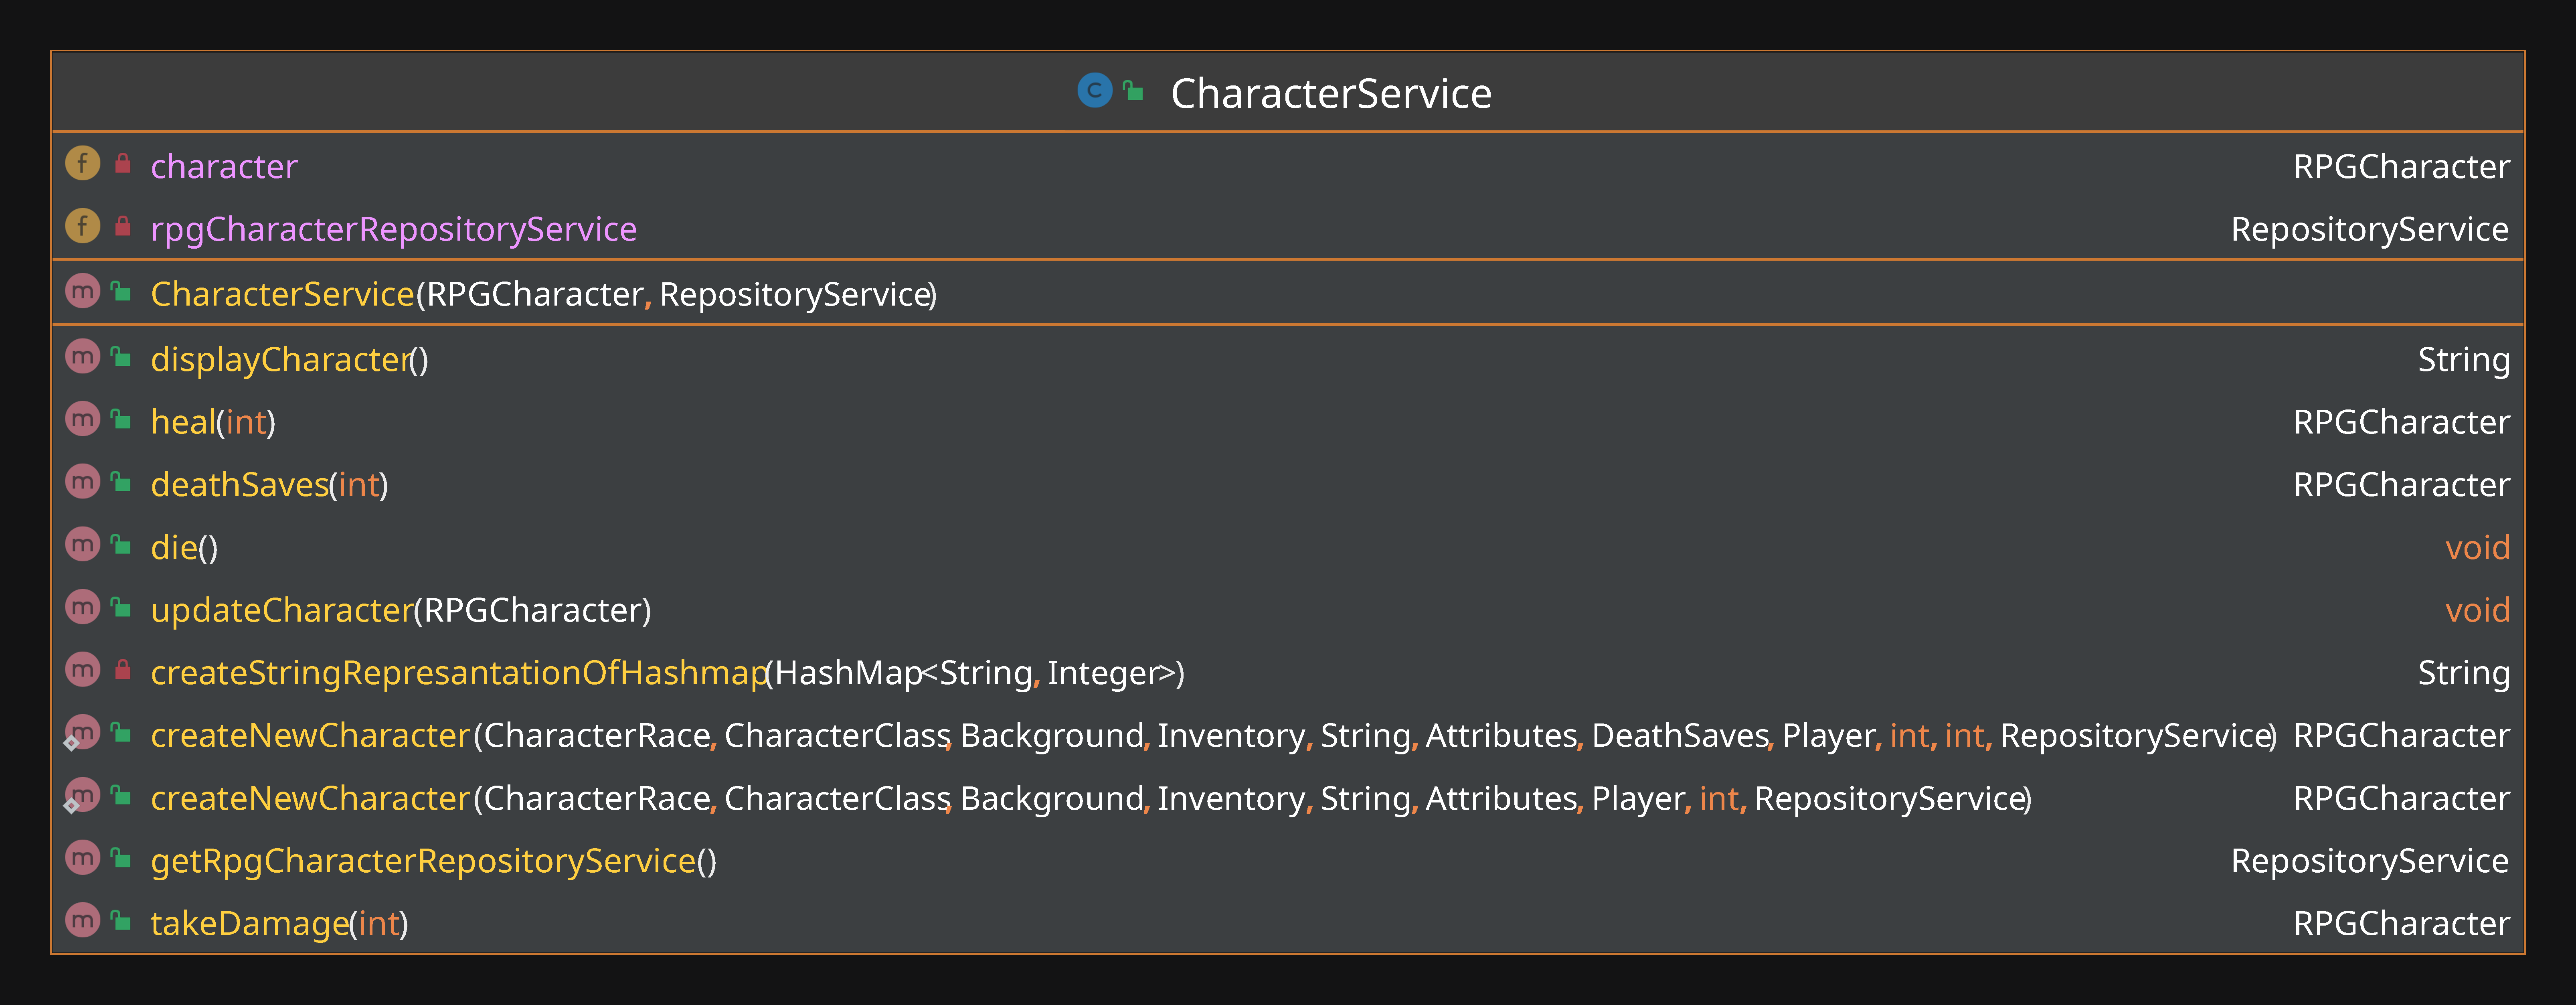
\includegraphics[width=0.49\textwidth]{Bilder/CharacterService.pdf}
	\caption{UML Diagramm des Character Service vor und nach dem Refactoring}
	\label{fig:rename}
\end{figure}
Die Methode \texttt{displayHashmap} wurde in \texttt{createStringRepresantationOfHashmap} umbennant, da die Methode keine Hashmap darstellt, sondern eine Stringrepräsentation einer übergebenen Hashmap baut und zurück gibt. Die UML Diagramme sind in Abbildung \ref{fig:rename} dargestellt. Alter commit: \href{https://github.com/lkno0705/DnD-CharacterManager/blob/497c202ebeea385178f9d1bca4aeb3401d92619c/2-dnd-charactermanager-application/src/main/java/character/CharacterService.java}{https://github.com/lkno0705/DnD-CharacterManager/blob/497c202ebeea385178f9d1bca4aeb3401d92619c/2-dnd-charactermanager-application/src/main/java/character/CharacterService.java}. Neuer commit: \href{https://github.com/lkno0705/DnD-CharacterManager/blob/main/2-dnd-charactermanager-application/src/main/java/character/CharacterService.java}{https://github.com/lkno0705/DnD-CharacterManager/blob/main/2-dnd-charactermanager-application/src/main/java/character/CharacterService.java}

\subsection{Extract Method}
\begin{figure}[H]
	\centering
	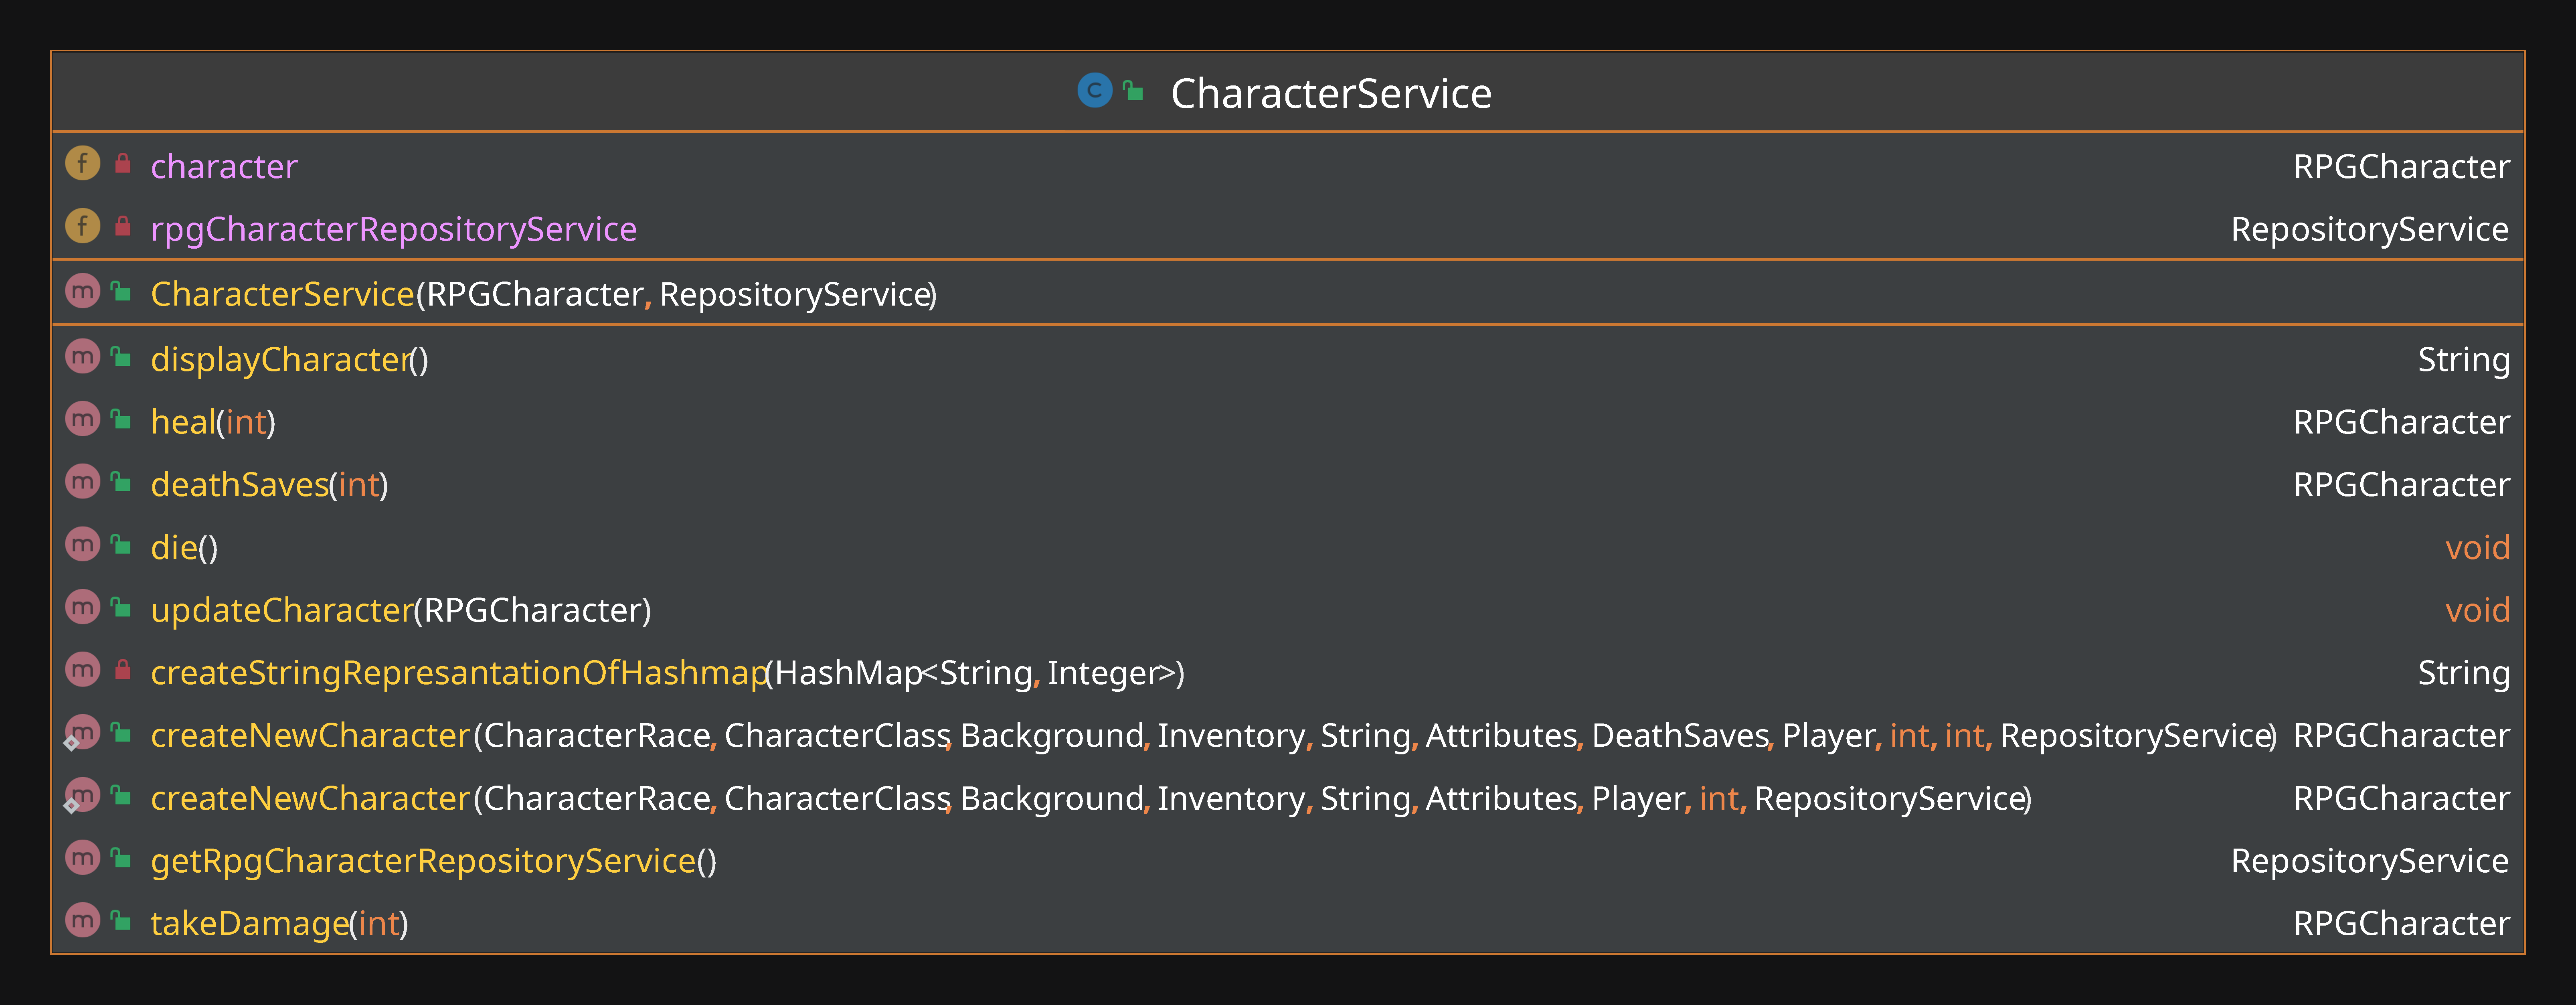
\includegraphics[width=0.49\textwidth]{Bilder/CharacterService.pdf}
	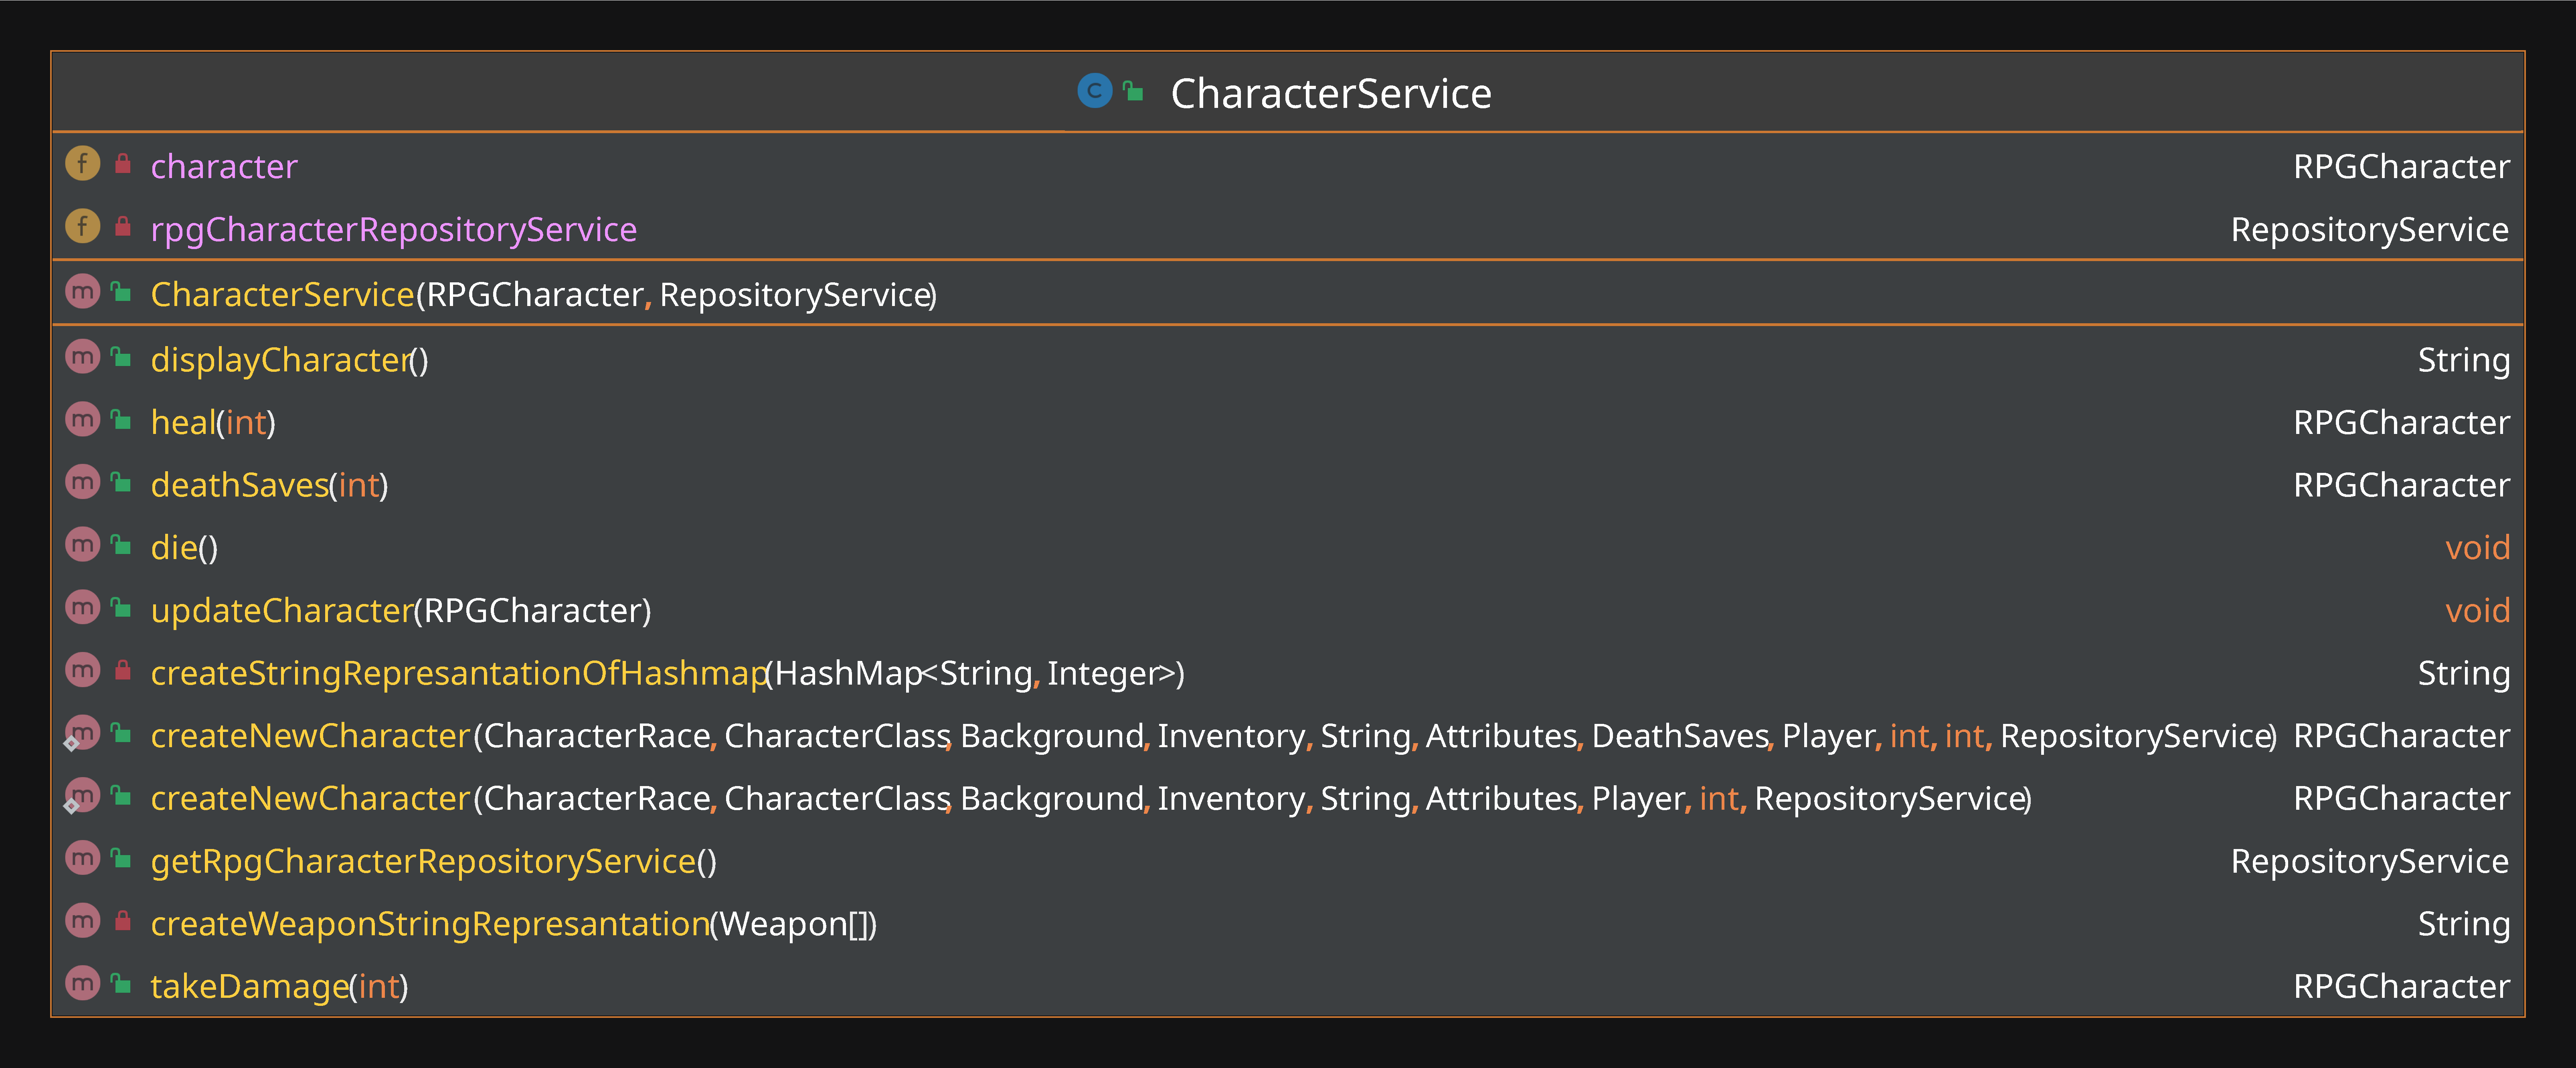
\includegraphics[width=0.49\textwidth]{Bilder/CharacterService-extracted.pdf}
	\caption{UML Diagramm des Character Service vor und nach dem Refactoring}
	\label{fig:extract}
\end{figure}
In der Methode \texttt{displayCharacter}, wurde eine \texttt{for-Schleife} extrahiert, die eine String Repräsentation des Waffen arrays des Inventorys aufgebaut hat. Dies dient dazu die recht lange Methode \texttt{displayCharacter} weiter zu verkürzen und so ihre lesbarkeit zu erhöhen.
